\section{Neutrino Oscillations. Theory}

%\subsection{Model of Two-Neutrino Oscillations in Vacuum}

Consider a simplified model of two-neutrino oscillations in vacuum as it is described in \cite{ref_Griffiths}, chapter 11. Suppose there are only two neutrinos: $\nu_e$ and $\nu_{\mu}$. Then energy eigenstates of the system would be the orthogonal combinations of neutrino flavor eigenstates:\\ 
\begin{center}
$\nu_1=\nu_{\mu}cos\theta-\nu_esin\theta$,\\ 
$\nu_2=\nu_{\mu}sin\theta+\nu_ecos\theta$.\\ 
\end{center}
Then, according to the quantum mechanics:\\ 
\begin{center}
$\nu_1(t)=\nu_1(0)e^{\frac{-iE_1t}{\hbar}}$, $\nu_2(t)=\nu_2(0)e^{\frac{-iE_2t}{\hbar}}$.\\ 
\end{center}
Suppose $\nu_e(t=0)=1$, $\nu_\mu(t=0)=0$. Then:\\ 
\begin{center}
$\nu_1(0)=-sin\theta$, $\nu_2(0)=cos\theta$,\\
$\nu_1(t)=-{sin\theta}e^{\frac{-iE_1t}{\hbar}}$, $\nu_2(t)={cos\theta}e^{\frac{-iE_2t}{\hbar}}$.\\ 
\end{center}
Thus, we obtain the system:\\ 
\begin{center}
$-{sin\theta}e^{-{{iE_1t} \over \hbar}}=\nu_\mu(t)cos\theta-\nu_e(t)sin\theta$,\\
${cos\theta}e^{-{{iE_2t} \over \hbar}}=\nu_\mu(t)sin\theta+\nu_e(t)cos\theta$.\\ 
\end{center}
By solving this system for $\nu_e$ and $\nu_\mu$, one obtains:\\ 
\begin{center}
\begin{equation}
\label{eq:P_twoNu1}
P_{\nu_e \rightarrow \nu_\mu} = |\nu_\mu(t)|^2=[{sin2\theta}sin{\frac{(E_1-E_2)t}{2\hbar}}]^2,
\end{equation}
\begin{equation}
\label{eq:P_twoNu2}
P_{\nu_e \rightarrow \nu_e}=|\nu_e(t)|^2=1-[{sin2\theta}sin{\frac{(E_1-E_2)t}{2\hbar}}]^2.
\end{equation}
\end{center}
According to Formulas \ref{eq:P_twoNu1} and \ref{eq:P_twoNu2}, for freely traveling neutrinos, if $\nu_e$ was emitted, at any point there is a certain probability to register $\nu_e$ or $\nu_\mu$, and those probabilities change with time periodically, according to the $~[sin(At)]^2$ law. That is why the phenomenon is called the neutrino oscillations.
Suppose momenta $p_1=p_2$. Then using $E^2=p^2+m^2$ and assuming $m_{1,2}\ll E_{1,2}$, the probabilities will take forms of:\\
\begin{center}
\begin{equation}
\label{eq:P_twoNu3}
P_{\nu_e \rightarrow \nu_\mu}=|\nu_\mu(t)|^2=[{sin2\theta}sin{\frac{(E_1-E_2)t}{2\hbar}}]^2=[{sin2\theta}sin{\frac{(m_1^2-m_2^2)c^3}{4\hbar{E}}z}]^2,
\end{equation}
\begin{equation}
\label{eq:P_twoNu4}
P_{\nu_e \rightarrow \nu_e}=|\nu_e(t)|^2=1-[{sin2\theta}sin{\frac{(m_1^2-m_2^2)c^3}{4\hbar{E}}z}]^2.
\end{equation}
\end{center}
Therefore, for neutrino oscillations to be present in the two-neutrino system,  neutrino mixing must be present ($\theta \neq 0$), and at least one of two neutrinos must be massive, satisfying $m_2 \neq m_1$.\\ \\
%\subsection{Mechanism of Neutrinos Getting Mass}
Neutrinos were believed to be massless for a long time, and the simplified weak interactions theory introduces Lagrangian with massless neutrinos \cite{ref_Griffiths}. Experiments for direct neutrino mass measurements were only able to set upper limits on the neutrino masses. However, the neutrino oscillations were experimentally observed and therefore at least two out of three neutrinos must be massive. \\ \\
There are two the most commonly discussed mechanisms of giving neutrinos mass in the Standard Model: one assumes neutrinos to be Dirac particles ($\nu \neq \bar{\nu}$), and the other one assumes neutrinos to be Majorana particles ($\nu = \bar{\nu}$) \cite{ref_PDG}, \cite{ref_theory_Osc}. If the neutrinos are Dirac, both left-handed and right-handed neutrinos must be present in the Standard Model Lagrangian, but the right-handed neutrino term would be significantly suppressed. Only left-handed neutrinos have been experimentally observed to date which is consistent with an assumption that right-handed neutrinos can participate in weak interactions but with a much smaller probability than left-handed neutrinos. If the neutrinos are Majorana, there is no need for the right-handed neutrino term in the Lagrangian. Majorana neutrinos would mean that there is no lepton flavor number conservation, but lepton flavor number has been observed to be conserved in all phenomena except neutrino oscillations. \\ \\
In the remaining portion of this chapter we consider the three-neutrino mixing matrix and $P_{\nu_\mu \rightarrow \nu_e}$ in the presence of three neutrinos in the Dirac neutrino case.\\ \\ 
%\subsection{Three-Neutrino Oscillation}
Three-neutrino case is described in \cite{ref_theory_Osc} and \cite{ref_LBNF_CDR}. For three-neutrino case, the oscillations are determined by a complex unitary matrix which is called Pontecorvo-Maki-Nakagava-Sakata (PMNS) matrix:\\ \\
\begin{center}
$ \begin{pmatrix} \nu_{e} \\ \nu_{\mu} \\ \nu_{\tau} \\ \end{pmatrix}
 = U_{PMNS}\cdot \begin{pmatrix} \nu_{1} \\ \nu_{2} \\ \nu_{3} \\ \end{pmatrix} = 
 \begin{pmatrix}
  U_{e1} & U_{e2} & U_{e3} \\
  U_{\mu1} & U_{\mu2} & U_{\mu3} \\
  U_{\tau1} & U_{\tau2} & U_{\tau3} \\
 \end{pmatrix}
 \cdot
\begin{pmatrix} \nu_{1} \\ \nu_{2} \\ \nu_{3} \\ \end{pmatrix}$.\\
\end{center}
An arbitrary 3x3 unitary matrix can be parametrized by 9 parameters, but 5 of them can be absorbed as Dirac phases which do not change the physical properties of the system and therefore the $U_{PMNS}$ matrix can be parametrized with three neutrino mixing angles ($\theta_{12}$, $\theta_{23}$, $\theta_{13}$) and one complex phase $\delta$. If we define $c_{ab}=cos\theta_{ab}$, $s_{ab}=sin\theta_{ab}$, the $U_{PMNS}$ matrix can be split into three multipliers:\\ 
\begin{center}
$U_{PMNS} =
 \begin{pmatrix}
  1 & 0 & 0 \\
  0 & c_{23} & s_{23} \\
  0 & -s_{23} & c_{23} \\
 \end{pmatrix}
 \cdot
 \begin{pmatrix}
  c_{13} & 0 & e^{i\delta}s_{13} \\
  0 & 1 & 0 \\
  -e^{i\delta}s_{13} & 0 & c_{13} \\
 \end{pmatrix}
 \cdot
 \begin{pmatrix}
  c_{12} & s_{12} & 0 \\
  -s_{12} & c_{12} & 0 \\
  0 & 0 & 1 \\
 \end{pmatrix}$. \\
\end{center}
Probability $P_{\nu_\mu \rightarrow \nu_e}$ in three-neutrino model in vacuum is given by Formula \ref{eq:P_noMatter} (\cite{ref_theory_Osc}): \\ \\
\begin{center}
\begin{equation}
\label{eq:P_noMatter}
P_{\nu_\mu \rightarrow \nu_e} \simeq P_1 + P_2 + P_3, 
\end{equation}
\begin{equation}
\label{eq:P_noMatter_1}
P_1 = sin^2{\theta_{23}} \cdot sin^2{2\theta_{13}} \cdot sin^2{\Delta_{13}},
\end{equation}
\begin{equation}
\label{eq:P_noMatter_2}
P_2 = sin2\theta_{23} \cdot sin2\theta_{13} \cdot sin2\theta_{12} \cdot sin{\Delta_{31}} \cdot \Delta_{21} \cdot cos(\Delta_{32}+\delta),
\end{equation}
\begin{equation}
\label{eq:P_noMatter_3}
P_3 = cos^2\theta_{23} \cdot cos^2\theta_{31} \cdot sin^2{2\theta_{12}} \cdot \Delta^2_{21},
\end{equation}
\end{center}
where $\Delta_{ij}={\Delta}m^2_{ij}L/4E$, E is a neutrino energy, and L is a distance traveled by neutrino after being produced (a baseline).\\ \\
Therefore, $P_{\nu_\mu \rightarrow \nu_e}$ depends on the $U_{PMNS}$ parameters, and the differences of squares of neutrino masses. There are two independent expressions for squares of the mass differences: ${\Delta}m_{21}^2 = m_2^2-m_1^2$ and ${\Delta}m_{32}^2 = m_3^2-m_2^2$. The mixing angles $\theta_{12}$, $\theta_{23}$, $\theta_{13}$ have been measured experimentally, and give the $U_{PMNS}$ matrix a form of:\\
\begin{center}
$|U_{PMNS}| \sim
 \begin{pmatrix}
  0.8 & 0.5 & 0.2 \\ 0.5 & 0.6 & 0.6 \\ 0.2 & 0.6 & 0.8 \\
 \end{pmatrix}$.\\
\end{center}
The phase $\delta$ is unknown.\\ \\
The analogous matrix for quark mixing, Cabibbo-Kobayashi-Maskawa (CKM) matrix $V_{CKM}$, is much more diagonal:\\
\begin{center}
$|V_{CKM}| \sim
 \begin{pmatrix}
  1 & 0.2 & 0.004 \\ 0.2 & 1 & 0.04 \\ 0.008 & 0.04 & 1 \\
 \end{pmatrix}$.\\
\end{center}
One important question in modern particle physics is why the quark mixing angles are so much smaller than neutrino mixing angles, and whether there is any relationship between quark and neutrino mixing matrices.\\ \\
Overall, precision measurements of neutrino mixing parameters can bring an insight into understanding of fundamental particle physics questions.\\ \\
Wave functions of particles and antiparticles are complex conjugates to each other, and a presence of the non-zero complex phase $\delta$ in the mixing matrix would mean different behavior for $\nu_\mu \rightarrow \nu_e$ and $\bar{\nu_\mu} \rightarrow \bar{\nu_e}$ systems. If $\delta \neq 0$ then charge-spacial parity (CP) violation is present in the neutrino system. Because the $U_{PMNS}$ mixing matrix involves CP-violating phase, the studies of neutrino oscillations could provide a hint into the origin of matter-antimatter asymmetry in the Universe. When the Universe was created after the Big Bang, there was supposed to be equal amount of matter and antimatter. Then most of matter and antimatter annihilated, and the tiny excess of matter created the whole Universe which we have today. One possible explanation of an origin of this tiny excess is CP-violation. It is experimentally known that electromagnetic and strong interactions conserve CP, and it only can be violated in the weak interactions. CP-violation in the quark sector has been observed experimentally, and it can also present in the lepton sector due to $\delta$ phase in the neutrino mixing matrix. But neutrino oscillation experiments performed before were not sensitive enough to measure $\delta$.\\ \\
Precision measurements of the parameters of the $U_{PMNS}$ matrix and comparing it to the $V_{CKM}$ matrix may help understanding whether there is any relationship between quark and neutrino mixing. One especially interesting parameter of the $U_{PMNS}$ matrix is angle $\theta_{23}$. According to currently available experimental results, it is indistinguishable from $45^0$($sin^2(2\theta_{23})=0.999^{+0.001}_{-0.018}$ \cite{ref_PDG}). If $\theta_{23}=45^0$ exactly, it might be an indication of a new, unknown symmetry.\\ \\
Mass differences were measured in other neutrino oscillation experiments, but ${\Delta}m_{21}^2$ and ${\Delta}m_{32}^2$ are present in Formula \ref{eq:P_noMatter} evenly and therefore neutrino oscillations in vacuum are not sensitive to the signs of these expressions. Ordering of neutrino masses is called mass hierarchy (MH). Determining mass hierarchy can bring an insight into understanding the flavor symmetry. All the higher generation quarks and charged leptons have higher masses than corresponding lower generation particles (Fig. \ref{fig:StandardModel}), and only ordering of neutrino masses is not known. If the neutrino MH will be found to be $m_3>m_2>m_1$, that would mean that masses of all the fundamental particles order the same way from generation to generation. \\
$P_{\nu_\mu \rightarrow \nu_e}$ in presence of matter assuming it has constant density is described by Formula \ref{eq:P_bigFormula} \cite{ref_theory_Osc}: \\
\begin{center}
\begin{equation}
\label{eq:P_bigFormula}
P_{\nu_\mu \rightarrow \nu_e} \simeq P_1 + P_2 + P_3, 
\end{equation}
\begin{equation}
\label{eq:P_bigFormula_1}
P_1 = sin^2{\theta_{23}} \cdot sin^2{2\theta_{13}} \cdot \frac{sin^2(\Delta_{13}-aL)}{(\Delta_{13}-aL)^2} \cdot \Delta^2_{31},
\end{equation}
\begin{equation}
\label{eq:P_bigFormula_2}
P_2 = sin2\theta_{23} \cdot sin2\theta_{13} \cdot sin2\theta_{12} \cdot \frac{sin(\Delta_{31}-aL)}{(\Delta_{31}-aL)} \cdot \Delta_{31} \cdot \frac{sin(aL)}{aL}\Delta_{21} \cdot cos(\Delta_{31}+\delta),
\end{equation}
\begin{equation}
\label{eq:P_bigFormula_3}
P_3 = cos^2\theta_{23} \cdot sin^2{2\theta_{12}} \cdot \frac{sin^2(aL)}{(aL)^2} \cdot \Delta^2_{21},
\end{equation}
\end{center}
where $a={G_F}{N_e}/\sqrt{2}$, $G_F$ is the Fermi constant, $N_e$ is a number density of electrons in the Earth's matter, and L is a baseline.\\ \\
For $P(\bar{\nu_\mu} \rightarrow \bar{\nu_e})$ one would need to change $\delta \rightarrow -\delta$ and $a \rightarrow -a$ \cite{ref_theory_Osc}. The $a \rightarrow -a$ effect introduces sensitivity to MH, and increases with L. It was determined that $m_2>m_1$ however the sign of ${\Delta}m_{32}^2$ is unknown. If the masses order as $m_3 > m_2 > m_1$ it is called normal neutrino mass hierarchy (NH), and if the masses order as $m_2 > m_1 > m_3$ it is called inverted neutrino mass hierarchy (IH).\\ \\
Fig. \ref{fig:LBNF_oscProbability} shows $P_{\nu_\mu \rightarrow \nu_e}$ at a baseline of L=1300 km. Magnitude and frequency of oscillations both depend on $\delta$, and the differences become more significant for higher oscillation nodes which correspond to lower neutrino/antineutrino energies. Changes due to different values of $\delta$ are opposite for neutrinos and antineutrinos.\\ \\
\begin{figure}
\caption{$P(\nu_\mu \rightarrow \nu_e)$ at a baseline of 1300 km, as a function of neutrino energy. Left: neutrinos, right: antineutrinos. Source of figure: \cite{ref_LBNF_CDR}.}
\label{fig:LBNF_oscProbability}
\centering
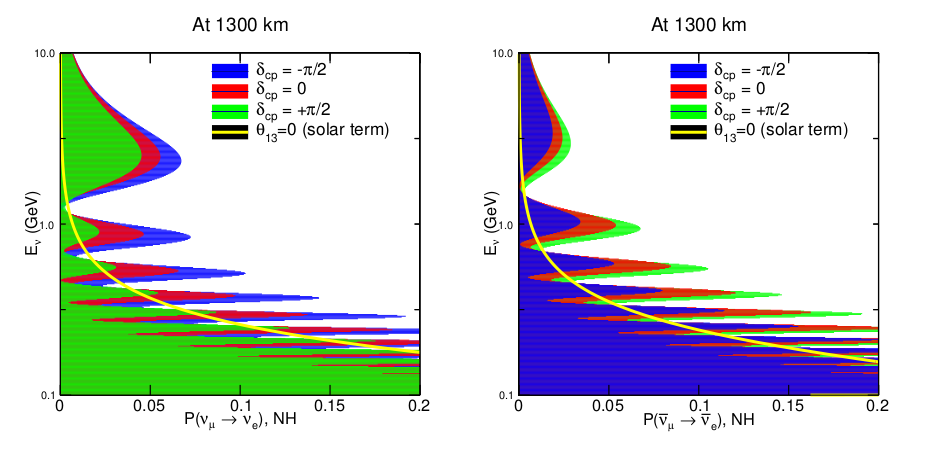
\includegraphics[width=0.98\textwidth, keepaspectratio=true]{figs/LBNF_oscProbability.png} 
\end{figure}

